%%
%% This is file `sample-sigconf.tex',
%% generated with the docstrip utility.
%%
%% The original source files were:
%%
%% samples.dtx  (with options: `all,proceedings,bibtex,sigconf')
%%
%% IMPORTANT NOTICE:
%%
%% For the copyright see the source file.
%%
%% Any modified versions of this file must be renamed
%% with new filenames distinct from sample-sigconf.tex.
%%
%% For distribution of the original source see the terms
%% for copying and modification in the file samples.dtx.
%%
%% This generated file may be distributed as long as the
%% original source files, as listed above, are part of the
%% same distribution. (The sources need not necessarily be
%% in the same archive or directory.)
%%
%%
%% Commands for TeXCount
%TC:macro \cite [option:text,text]
%TC:macro \citep [option:text,text]
%TC:macro \citet [option:text,text]
%TC:envir table 0 1
%TC:envir table* 0 1
%TC:envir tabular [ignore] word
%TC:envir displaymath 0 word
%TC:envir math 0 word
%TC:envir comment 0 0
%%
%%
%% The first command in your LaTeX source must be the \documentclass
%% command.
%%
%% For submission and review of your manuscript please change the
%% command to \documentclass[manuscript, screen, review]{acmart}.
%%
%% When submitting camera ready or to TAPS, please change the command
%% to \documentclass[sigconf]{acmart} or whichever template is required
%% for your publication.
%%
%%
\documentclass[bibtex, sigconf, hyperref={colorlinks=true,linkcolor=blue,urlcolor=blue}]{acmart}

%%
%% \BibTeX command to typeset BibTeX logo in the docs
\AtBeginDocument{%
  \providecommand\BibTeX{{%
    Bib\TeX}}}

%% Rights management information.  This information is sent to you
%% when you complete the rights form.  These commands have SAMPLE
%% values in them; it is your responsibility as an author to replace
%% the commands and values with those provided to you when you
%% complete the rights form.

% Is this necessary for us?
\setcopyright{acmlicensed}
\copyrightyear{2024}
\acmYear{2024}
\acmDOI{XXXXXXX.XXXXXXX}

%% These commands are for a PROCEEDINGS abstract or paper.
% \acmConference[Conference acronym 'XX]{Make sure to enter the correct
%   conference title from your rights confirmation emai}{June 03--05,
%   2018}{Woodstock, NY}
%%
%%  Uncomment \acmBooktitle if the title of the proceedings is different
%%  from ``Proceedings of ...''!
%%
%%\acmBooktitle{Woodstock '18: ACM Symposium on Neural Gaze Detection,
%%  June 03--05, 2018, Woodstock, NY}
% \acmISBN{978-1-4503-XXXX-X/18/06}


%%
%% Submission ID.
%% Use this when submitting an article to a sponsored event. You'll
%% receive a unique submission ID from the organizers
%% of the event, and this ID should be used as the parameter to this command.
%%\acmSubmissionID{123-A56-BU3}

%%
%% For managing citations, it is recommended to use bibliography
%% files in BibTeX format.
%%
%% You can then either use BibTeX with the ACM-Reference-Format style,
%% or BibLaTeX with the acmnumeric or acmauthoryear sytles, that include
%% support for advanced citation of software artefact from the
%% biblatex-software package, also separately available on CTAN.
%%
%% Look at the sample-*-biblatex.tex files for templates showcasing
%% the biblatex styles.
%%

%%
%% The majority of ACM publications use numbered citations and
%% references.  The command \citestyle{authoryear} switches to the
%% "author year" style.
%%
%% If you are preparing content for an event
%% sponsored by ACM SIGGRAPH, you must use the "author year" style of
%% citations and references.
%% Uncommenting
%% the next command will enable that style.
%%\citestyle{acmauthoryear}


%%
%% end of the preamble, start of the body of the document source.
\begin{document}

%%
%% The "title" command has an optional parameter,
%% allowing the author to define a "short title" to be used in page headers.
\title{Predictors of NFL tackles}

%%
%% The "author" command and its associated commands are used to define
%% the authors and their affiliations.
%% Of note is the shared affiliation of the first two authors, and the
%% "authornote" and "authornotemark" commands
%% used to denote shared contribution to the research.
\author{Isaac Kou (4502)}
\email{Isaac.Kou@colorado.edu}
\affiliation{%
  \institution{University of Colorado Boulder}
  \city{Boulder}
  \state{Colorado}
  \country{USA}
}

\author{Sean Shi (4502)}
\email{Sean.Shi@colorado.edu}
\affiliation{%
  \institution{University of Colorado Boulder}
  \city{Boulder}
  \state{Colorado}
  \country{USA}
}

\author{Timur Tripp (5502)}
\email{Timur.Tripp@colorado.edu}
\affiliation{%
  \institution{University of Colorado Boulder}
  \city{Boulder}
  \state{Colorado}
  \country{USA}
}

\author{Grace Williams (5502)}
\email{grwi3115@colorado.edu}
\affiliation{%
  \institution{University of Colorado Boulder}
  \city{Boulder}
  \state{Colorado}
  \country{USA}
}

% \authornote{Both authors contributed equally to this research.}
% \orcid{1234-5678-9012}
% \author{G.K.M. Tobin}
% \authornotemark[1]
% \affiliation{%
%   \institution{Institute for Clarity in Documentation}
%   \city{Dublin}
%   \state{Ohio}
%   \country{USA}
% }

%%
%% By default, the full list of authors will be used in the page
%% headers. Often, this list is too long, and will overlap
%% other information printed in the page headers. This command allows
%% the author to define a more concise list
%% of authors' names for this purpose.
\renewcommand{\shortauthors}{Isaac et al.}

%%
%% The abstract is a short summary of the work to be presented in the
%% article.

%%
%% The code below is generated by the tool at http://dl.acm.org/ccs.cfm.
%% Please copy and paste the code instead of the example below.
%%

%%
%% Keywords. The author(s) should pick words that accurately describe
%% the work being presented. Separate the keywords with commas.
\keywords{Football, NFL, Data Mining, Tackles}

%% A "teaser" image appears between the author and affiliation
%% information and the body of the document, and typically spans the
%% page.

\begin{teaserfigure}
% Random image of tackling I pulled from the internet, feel free to replace
  % \caption{Seattle Mariners at Spring Training, 2010.}
  % \Description{Enjoying the baseball game from the third-base
  % seats. Ichiro Suzuki preparing to bat.}
  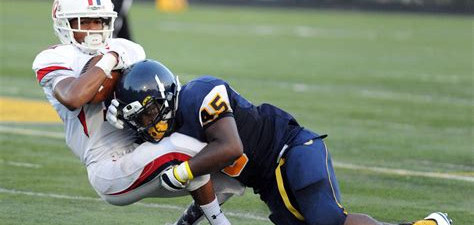
\includegraphics[width=\textwidth]{./th-4169371817}
  \label{fig:teaser}
\end{teaserfigure}

\received{27 September 2024}
% \received[revised]{12 March 2009}
% \received[accepted]{5 June 2009}

%%
%% This command processes the author and affiliation and title
%% information and builds the first part of the formatted document.
\maketitle

\section{Introduction}
Every year, the Nation Football league hosts the NFL Big Data Bowl, a yearly sports data analytics competition in which teams analyze specific datasets provided by Next Gen Stats in order to encourage data-backed improvements to the NFL. The data, which aligns with the competition's yearly theme, is
\begin{quote}
\textit{``the capture of real time location data, speed and acceleration for every player, every play on every inch of the field. Sensors throughout the stadium track tags placed on players' shoulder pads, charting individual movements within inches."}

\cite{nextgenstats}
% \raggedleft{[Next Gen Stats, 2024 \url{https://nextgenstats.nfl.com/glossary}]}
\end{quote}
Specifically, the 2024 Big Data Bowl focuses on the theme of tackling in order to encourage the creation of metrics quantifying things like tackle probability, play impacts, expected points, and injury.

Tackling is imperative to the sport of American football, as the defending team's main goal is to tackle the opposing player with the football as soon as possible in order to help prevent the team from scoring. As such, the dataset used to analyze tackling includes categories on game data, play data, player data, tackles data, and tracking data. The goal of this project is to utilize such metrics in order to find correlations between known information such as weight, height, and time during a game and the outcome of plays (whether or not the tackle was completed, whether the tackle was successful in terms of gameplay, etc.).

\section{Existing Work}
A significant number of previous academic studies exist on the topic of
tackling in American football. This section discusses three examples of those
studies, one hobbyist analysis, and the foundation they lay for our proposed
work.

The paper \href{https://link.springer.com/article/10.1007/s10439-020-02625-7}{“Validating Tackle
Mechanics in American Football: Improving Safety and Performance”}\cite{validatingtackles} (Maerlender et al.) discusses the
development of a program to reduce the risk of serious injury from tackling, specifically by identifying
head-contact likelihoods and therefore alternative techniques to reduce such contact. Secondary research
related to the impact of tackles on player performance was also conducted, finding a reduction in
their number of yards run post-contact.

Similarly, \href{https://www.jstage.jst.go.jp/article/ijshs/16/0/16_201804/_article/-char/ja/}
{“Effectiveness of the Heads Up Tackling (HUT) Program on Tackling Safety and Performance in American Football”}\cite{effectiveness}
(Matsuo et al.) also identifies a program to promote tackle safety, though this study focuses
on an existing program and its observed impacts. Results indicated that implementation of the
studied HUT Program reduced rate and severity of player injury, with no detriment, or, in some
cases, even benefit, to player performance.

Lastly, \href{https://bmjopensem.bmj.com/content/6/1/e000638.abstract}{“Quantitative and qualitative
analysis of head and body impacts in American 7v7 non-tackle football”}\cite{quantitative} (Jadischke et al.) used video
analysis to investigate the rate of head contact in the alternative non-tackle play style of
American football. In a similar vein to the above studies, this research found that non-tackle
football was associated with lower rates of head contact and therefore potentially lower rates of
injury, though further research is needed.

Outside of academia, many football fans conduct hobbyist analyses of their own, often
concerning points, player performance, game trends, and so on. An example of this is
the article \href{https://medium.com/@ezra.ford/tackling-metrics-with-big-data-0812b5ab65f0}{“Tackling Metrics with Big Data”}
by Ezra Ford on Medium. In addition to being a subject of interest in and of themselves,
these have applications in related sub-hobbies, such as sports betting and fantasy football,
and can help fans maximize their success in those activities.

As shown, the existing work on tackles in American football often concerns the implications of
tackling, instead of the ability to predict and understand when/where/how tackles happen.
Thus, our work intends to investigate these trends instead.

\section{Methodology}

In this project, we seek to find the effects of different attributes on the
success rate and time of tackles and subsequently, how tackles effects the outcome
of a game.
To this end, we will be employing a variety of statistical techniques covered in
both CSCI4502/5502 and from other classes.

\subsection{Datasets}
To analyze the effect of various traits of player, matches, and other factors on
the timing and a success rate of tackle, we will primarily be using data from
the Kaggle NFL Big Data Bowl
\cite{nflkaggle}
% \footnote{\url{https://www.kaggle.com/competitions/nfl-big-data-bowl-2024/data}}
specifically the files ``\verb|tackles.csv|'', ``\verb|games.csv|'',
``\verb|plays.csv|'' which contain data on the play, players, success, teams,
etc. involved in a tackle.
We will also be examining data from 9 weeks of tracking data (``\verb|tracking_week_[1-9].csv|'')
to determine the effects of factors such as position on the field or movement at the time of a tackle.

% TODO: Maybe move some of this to future analysis?
\subsection{Proposed Analysis}
Our primary goal for this project is to find correlations between previously
known information such as weight, height, and time during a game and the tackles
performed (location, likelihood of success and number of tackles). To this end,
we are proposing to try and find correlations between factors such as height and
weight of player and frequency and likelihood of success of tackles and
frequency analysis for examining which teams/players tend to engage in tackles.

% We are also seeking to do time series analysis with the classical time series
% model to analyze the trend between time during a game an frequency of
% tackles. Additionally, we will use similar techniques to see if there is any
% trend in the number of tackles per game over time, though due to the limited
% scope of this dataset, we may need to use other data sources.

In addition to this analysis, we also seek to analyze whether the risk of injury
from tackles can be reduced and how much of an impact tackles have on the
outcome of a game or visa versa. We will also seek to analyze the difference in
frequencies of tackles between different teams and positions.

\section{Accomplished Work}
\subsection{Distance Before Tackle}
By analyzing the frequency of \verb|yardsToGo|, we were able to determine that
the vast majority of tackles occurred at around 10 yards. This is likely because
10 yards is the starting point for each round. We also see more observations
less than 10 yards to go than greater meaning moving forward is much more likely than backwards.
% Negative yardage: More than 10 yards to go, meaning the previous play lost yards. This can happen from an offensive penalty, a QB sack, or a tackle in the backfield.
The slight increase observed at 15 or 20 yards to go is likely due to penalties as -5 or -10 yards are common penalties.

\begin{figure}[h]
  \centering
  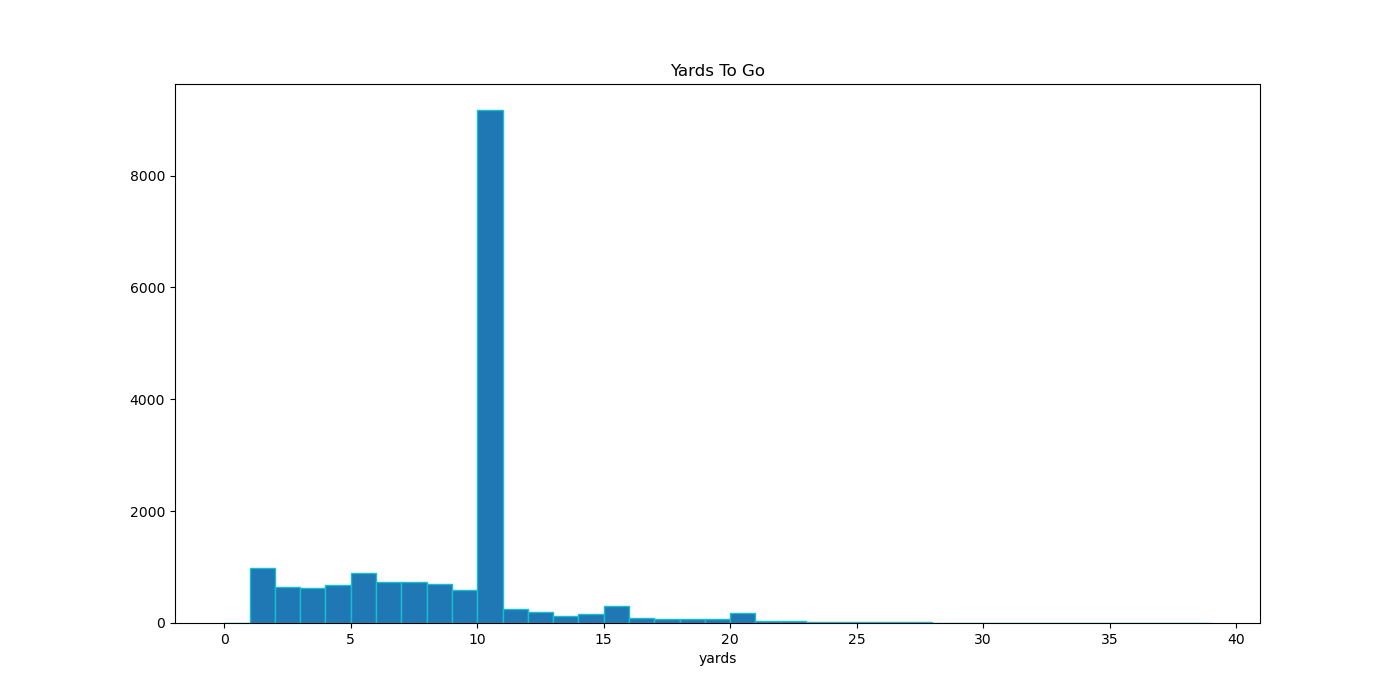
\includegraphics[width=\linewidth]{../src/yards.png}
  \caption{yards to go}
  \Description{A histogram of yards to go, has a peak at 10, more observations less than 10 than greater, and smaller peaks at 5, 10, -5, -10}
\end{figure}
\subsection{Predictor of Success}
To determine if certain factors about a player and the way a tackle was
performed made it more likely to succeed, we attempted to use a na\"ive
Bayesian classifier to predict the likelihood of a tackle succeeding based on
the following attributes:
\begin{itemize}
\item Weight: The player's height sorted into 3 categories: ($< 5'10'', 5'10''-6'2'', > 6'3''$)
\item Height: The player's weight sorted into 3 categories (`Under 200', `200 - 250', `Over 250')
\item Position: The player's position on the team (FB, QB, RB, TE, WR)
\item Assist: Whether or not the there were multiple people involved in the tackle
\item forcedFumble: Whether or not the ball was dislodged by the defender
\end{itemize}
These attributes were chosen because they were either intrinsic to the player
and likely meaningful to the game, or were dealt with how a tackle performed,
and thus could inform decisions about how to be more successful with future
tackles.

We used $70\%$ of the data for training the bayesian model and the rest for
testing its effectiveness in predicting success. The resulting model was able to
predict whether or not a tackle succeeded with accuracy of 88.6\% and F1 Score
of 0.8888216807787944. This shows that the factors chosen were effective in
predicting the likelihood of a tackle succeeding.

\subsection{Grouping tackles}
Examining 9 weeks of tracking data, we attempted to determine if there were any
patterns in where tackles occurred. This analysis used a subset of the tracking
data, specifically we filtered the dataset to only include the attributes for
the football and when a tackle occurred. We then used the $x$ and $y$ attributes
which correspond to the position of the football in yards at the time to the
tackle to determine if there any patterns in position. We attempted to use
k-means clustering with varying numbers of clusters to mine for clusters.

Our methods were unable to find significant clusters of positions where tackles
occurred. As shown in the figure below, the locations of tackles do not appear
to be in any statistically significant clusters. Notably, tackles tended to
occur much more frequently close to the center of the field in both the $x$ and
$y$ axes. One explanation for this is that players may be forced out of bounds
rather than tackled, which also ends the play.

\begin{figure}[h]
  \centering
  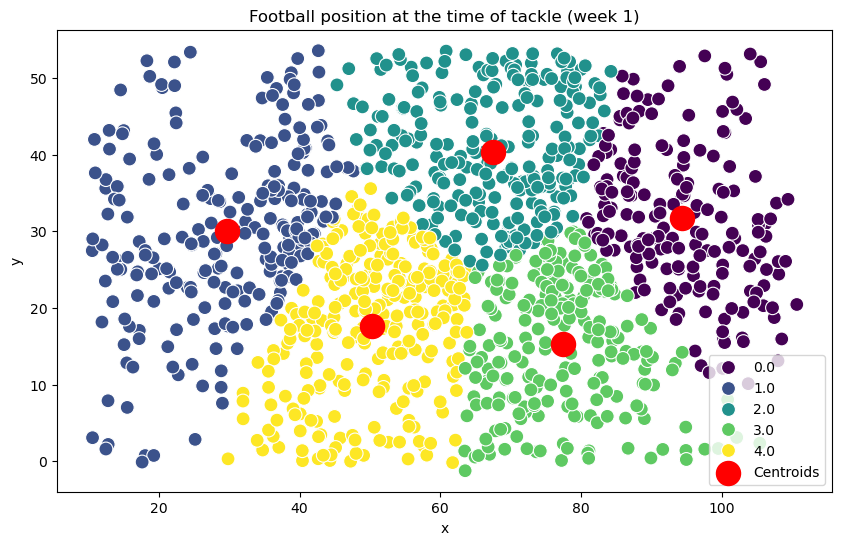
\includegraphics[width=\linewidth]{k-means}
  \caption{k-means analysis of week 1 data}
  \Description{A plot of the x and y coordinates of tackles in week 1 data}
\end{figure}

\section{Future Work}
Building off of the work done on predicting the likelihood of success of a
tackle, we plan to use different models with the same attributes and comparing
with the na\"ive Bayes results to see which is more accurate.
We plan on using a decision tree or random forest approach which should also
provide insight as to which attributes are most important in predicting
success.

In regards to the locations of tackles, we also plan to classify tackles as
success and failures to see if there are clusters where success or failure is
more likely.
Additionally, we also plan on looking into using other variables from the
tracking data such as speed and direction to determine if there are any
commonly occurring values for these variables.
We also plan on examining the data for outliers which may indicate that a
certain combination of attributes will make a tackle much more likely or less
likely to succeed.
Considering the role of defenders in a game, we also plan on examining if there
are certain strategies which allow the ball carrier to move past defenders.

Expanding analysis beyond looking at the likelihood of tackles succeeding,
we also plan on examining what impact tackles have on the course of the game.
We will try to find any events which are particularly important for the course
of the game using outlier analysis.
Additionally, we will see if the number of successful tackles has any effect on
which team will win the game.

\subsection{Not Currently in Scope}
We had considered using temporal data particularly the tracking data to see if
we can find any patterns over time. However, this may be difficult due to the
lack of historical data, short period of the tracking data, and its
incompleteness i.e. only including a few frames around each notable event in the
game.

\section{Evaluation}

As with any form of data analysis, we aim to find meaningful patterns and trends
that can illuminate bigger truths about our area of study without unwarranted
manipulation. Additionally, in order to conclude that these patterns and trends are
in fact meaningful, we must be able to disprove the null hypothesis.

In essence, if we are mining the data for the effect of an example X variable, the null
hypothesis would state that there is no statistical difference in tackle rate that can be
attributed to X variable, and that any observed difference is due to nothing more than chance.
Thus, in order to disprove it, the pattern would need to appear a sufficient amount of times
within the dataset to surpass the significance level (typically set at 5\%).

Notably, this is not the same as \textit{proving} the hypothesis. Rather, we will likely
only be able to disprove that it does not hold. This is often the case with real-world data,
and we will still be able to present our findings with some significance if that is the case.

In addition to these metrics, we will evaluate our work based on the thoroughness of our
investigation and our consideration of all factors. Real-world data is rarely straightforward,
and contains many confounding variables that can all have impacts on the observed results.
Accordingly, we will not necessarily make finding an “answer” our goal, but instead focus on
exploring the data as best we can.

\section{Milestones}
\begin{table}[H]
  \caption{Milestones for the semester}
  \label{tab:freq}
  \begin{tabular}{c|l}
    \toprule
    Date & Milestone \\
    \midrule
    9/24 - 9/26   & Project Proposal \\
    10/1 - 10/3   & Data discovery and cleaning complete \\
    10/8 - 10/10  & Begin initial analysis \\
    11/5 - 11/7   & Project Checkpoint Report \\
    11/12 - 11/14 & Analysis Complete \\
    12/3 - 12/5   & Visualizations in final deliverable form \\
                  & Summarize findings \\
    12/10 - 12/12 & Project Final Report \\
    \bottomrule
  \end{tabular}
\end{table}

\bibliographystyle{ACM-Reference-Format}
\bibliography{sources}
\nocite{*}

\end{document}
\endinput
